\beginsong{Weile an dieser Quelle}[
    wuw={Carl Michael Bellmann}, 
    txt={Carl Zuckmayer (Übersetzung)}, 
    bo={368},
]

\beginverse
\endverse
\centering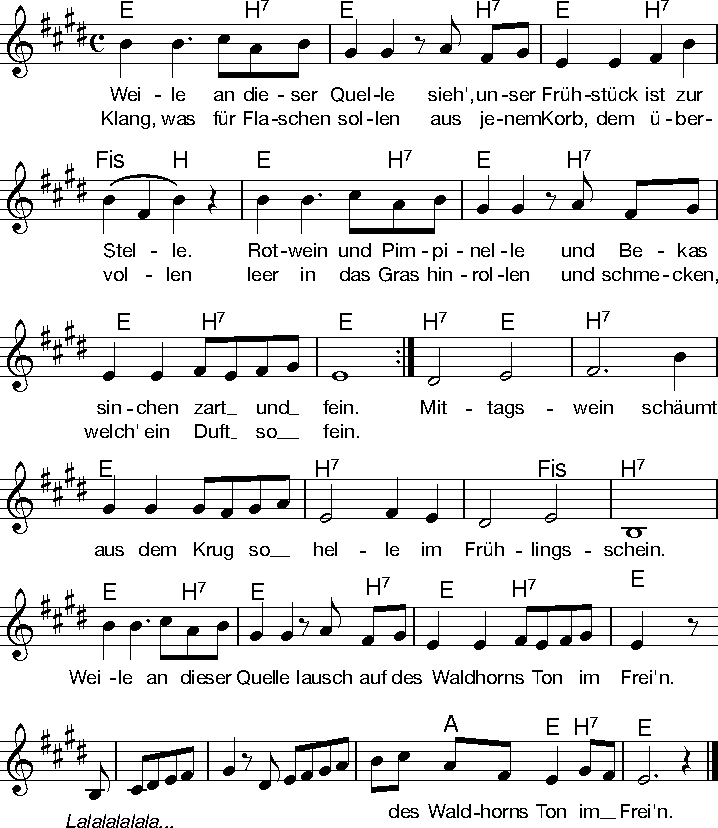
\includegraphics[width=1\textwidth]{Noten/Lied093a.pdf}

\beginverse
\endverse

\beginverse
\[E]Seht, wie das \[H7]Nymphlein \[E]eilet und \[H7]wie ihr \[E]Füßlein \[H7]nimmer \[F#]wei\[H]let,
\[E]Ei und \[H7]Oliv zer\[E]teilet und \[H7]schwitzt im \[E]eifri\[H7]gen Plai\[E]sir.
Seht wie ihr \[H7]Brüstlein \[E]hüpfet und \[H7]sich ihr \[E]Rock beim \[H7]Bücken \[F#]lüf\[H]tet,
\[E]ei, wie sie \[H7]dreist ent\[E]schlüpfet, fasst \[H7]man ans \[E]Knie und \[H7]höher \[E]ihr.
\[H7]Skoll, \[E]Ulla, \[H7]skoll. Lasst \[E]uns ein Schnäpslein \[H7]trinken, gestri\[F#]chen \[H7]voll,
\[E]dazu ein \[H7]Stückchen \[E]Schinken, das \[H7]uns vor\[E]trefflich \[H7]munden \[E]soll,
\echo{Lalalalalala... } das uns vor\[A]trefflich \[E]mun\[H7]den \[E]soll.
\endverse

\beginverse
^Spielet, ihr ^Musi^kanten, lasst ^Lied um ^Lied wie ^Schaum ^aufbran^den!
^Lachet der ^alten ^Tanten, die ^uns mit ^dürrem ^Finger ^dräu'n.
Schwirrt wie die ^nächt'gen ^Falter um ^unser ^Licht, ihr ^trunk'nen ^Psal^ter.
^Bald nacht sich ^graues ^Alter, drum ^lasst uns ^heut' der ^Lieder noch er^freu'n.
Viel ^Win^de ^weh'n von ^unbekannten ^Landen, Viel ^Jahre ^geh'n.
^Spielet, ihr ^Musi^kanten, lasst ^Lied um ^Lied wie ^Schaum auf^weh'n,
\echo{Lalalalalala... } lasst Lied um ^Lied wie ^Schaum ^auf^weh'n!
\endverse

\endsong

\beginscripture{}
Plaisir = Freude, Vergnügen
\endscripture
